\chapter{\textsc{Unité centrale}}

L'unité centrale ou CPU (Central Processing Unit) et le coeur du microcontrôleur. Elle effectue des opérations élémentaires sur des données ou sur des adresses. A l'intérieur du cpu on trouve une unité arithmétique et logique qu'on nomme ALU (Aritmetic and Logic Unit). c'est elle qui effectue les opérations de base tel que addition, multiplication, décalages et fonctions logiques. Pour qu'elle fonctionne optimalement, il faut l'alimenter avec des données de manière continue. Par la suite, on va détailler ce processus.

\section{Principes}

Un processeur se décompose en deux unités fondamentales: i) une unité de contrôle et ii) une unité de traitement  (fig. \ref{fig:cpu1}). L'unité de contrôle décode les instructions et pilote le chemin de données qui exécute les opérations. Le pilote du chemin de données s'appelle le séquenceur, il communique avec le chemin de données à l'aide de signaux de commande et reçois des informations sur son état. 

\begin{figure}[htb]
  \centering
  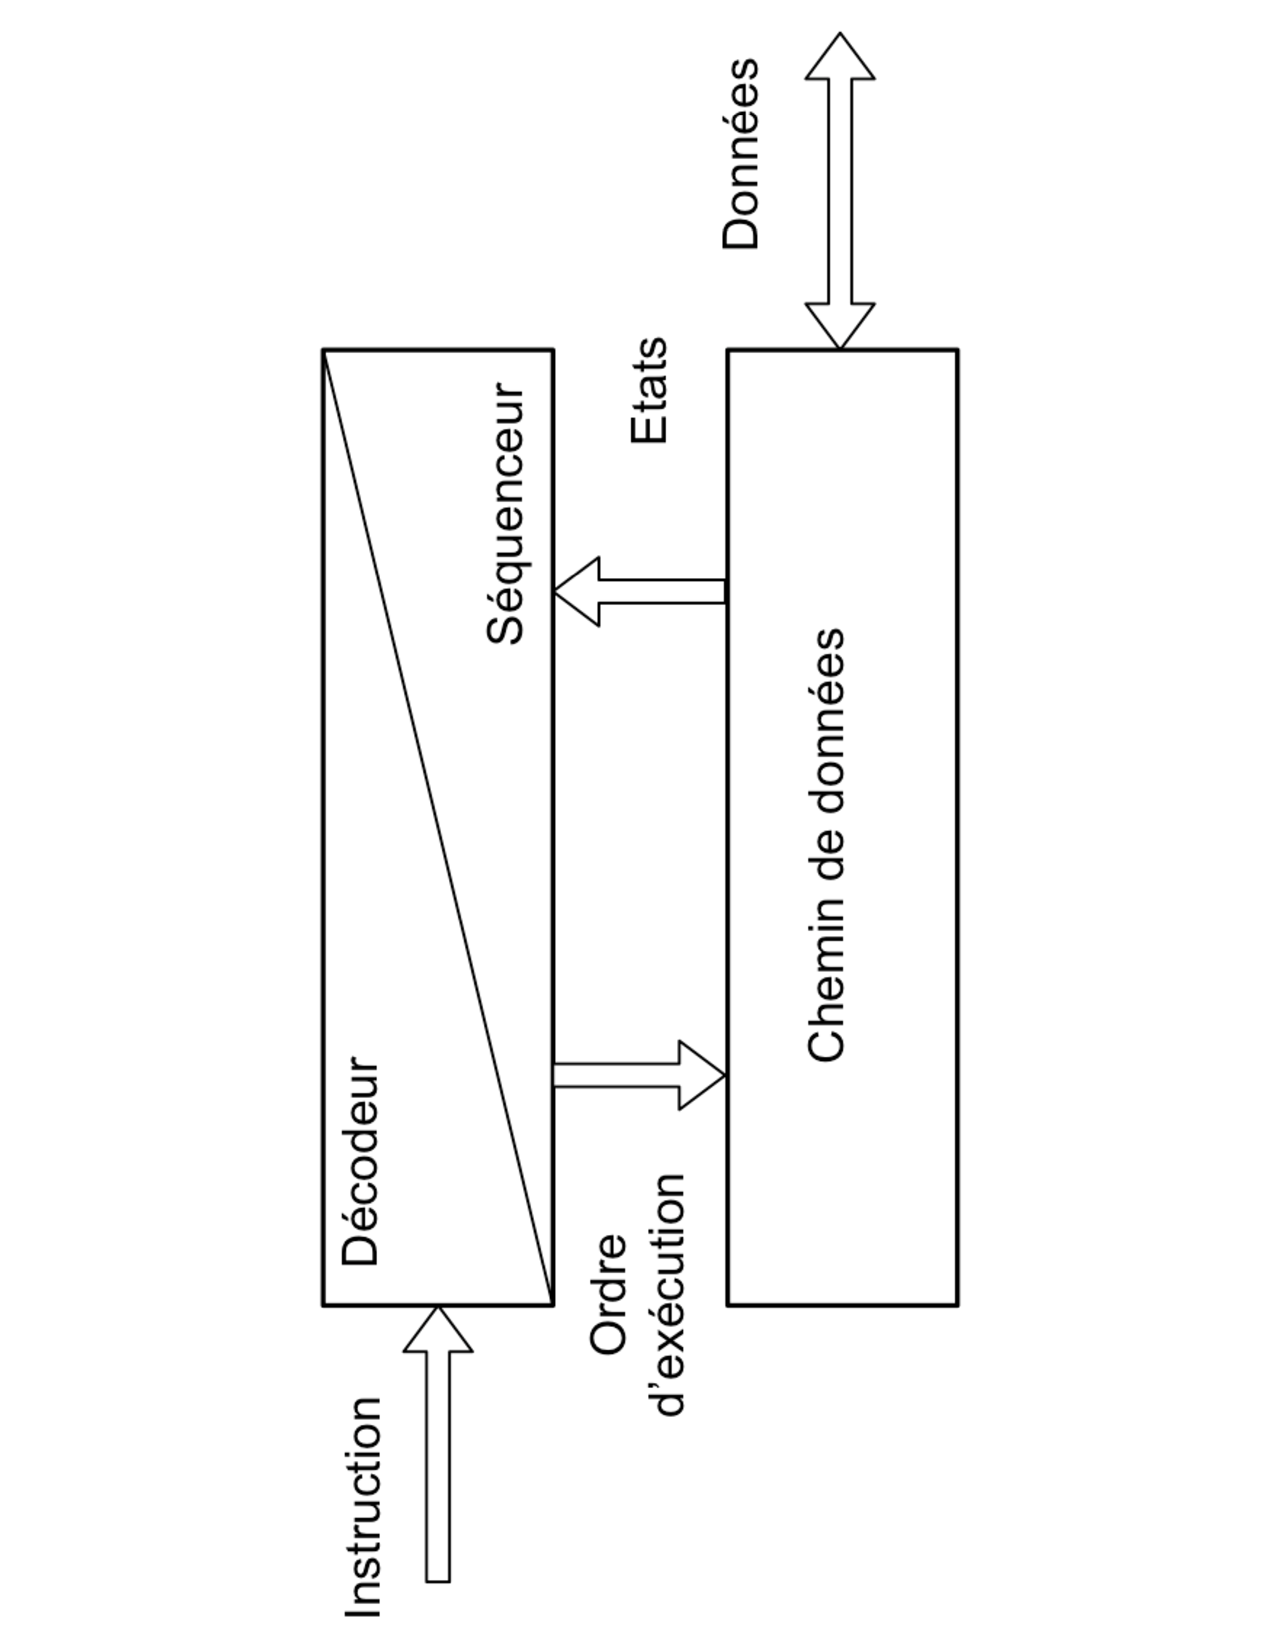
\includegraphics[angle=270, width=10cm,trim=100 1 100 1,clip]{./Figures/cpu/cpu1.pdf}
  \rule{35em}{0.5pt}
  \caption[cpu1]{Principe de fonctionnement de l'unité centrale}
  \label{fig:cpu1}
\end{figure}

Le chemin de donnée et l'unité de contrôle sont reliées par deux bus, le bus de données et le bus d'adresses (fig. \ref{fig:cpu2}). Le premier défini la largeur des mots traitables par le processeur (8, 16, 32 bits), le deuxième défini la taille mémoire adressable, par exemple: 16 bits = 65536 adresses.

\begin{figure}[htb]
  \centering
  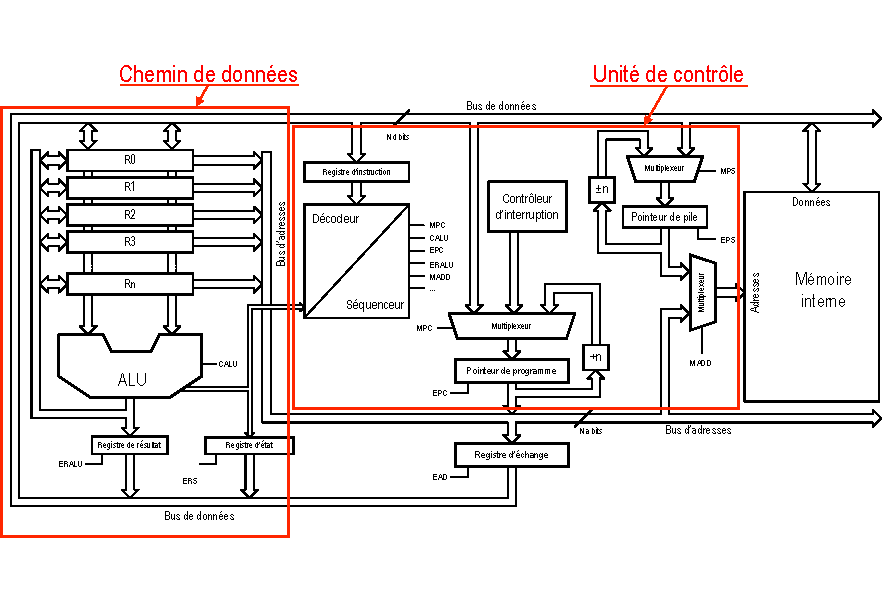
\includegraphics[angle=0, width=15cm, trim=0 20 0 30,clip]{./Figures/cpu/cpu2.pdf}
  \rule{35em}{0.5pt}
  \caption[cpu2]{Exemple d'unité centrale}
  \label{fig:cpu2}
\end{figure}

Le séquenceur est aussi responsable d'amener et de stocker des données dans la mémoire. On constate que le processeur à besoin de deux types d'information, les instructions et les données. Il y a donc deux possibilités, l'une ou l'on stock les deux informations dans une seule mémoire et l'autre ou on utilise deux mémoires séparées. Ce choix à provoqué une distinction importante en architecture des processeurs qu'on a nommé Von Neumann et Harvard.

\subsection{Architectures de Von Neumann et Harvard}
Cette différence de stockage des données et des instructions peut amener des avantages et des inconvénients. Si les données et les instructions sont séparées, il faut deux mémoires et deux bus d'accès. Par contre, si il y a deux mémoires, le chargement se fait en parallèle. On peut donc considérer que l'architecture de Von Neumann est plus simple mais moins performante que celle de Harvard.

\begin{figure}[htb]
  \centering
  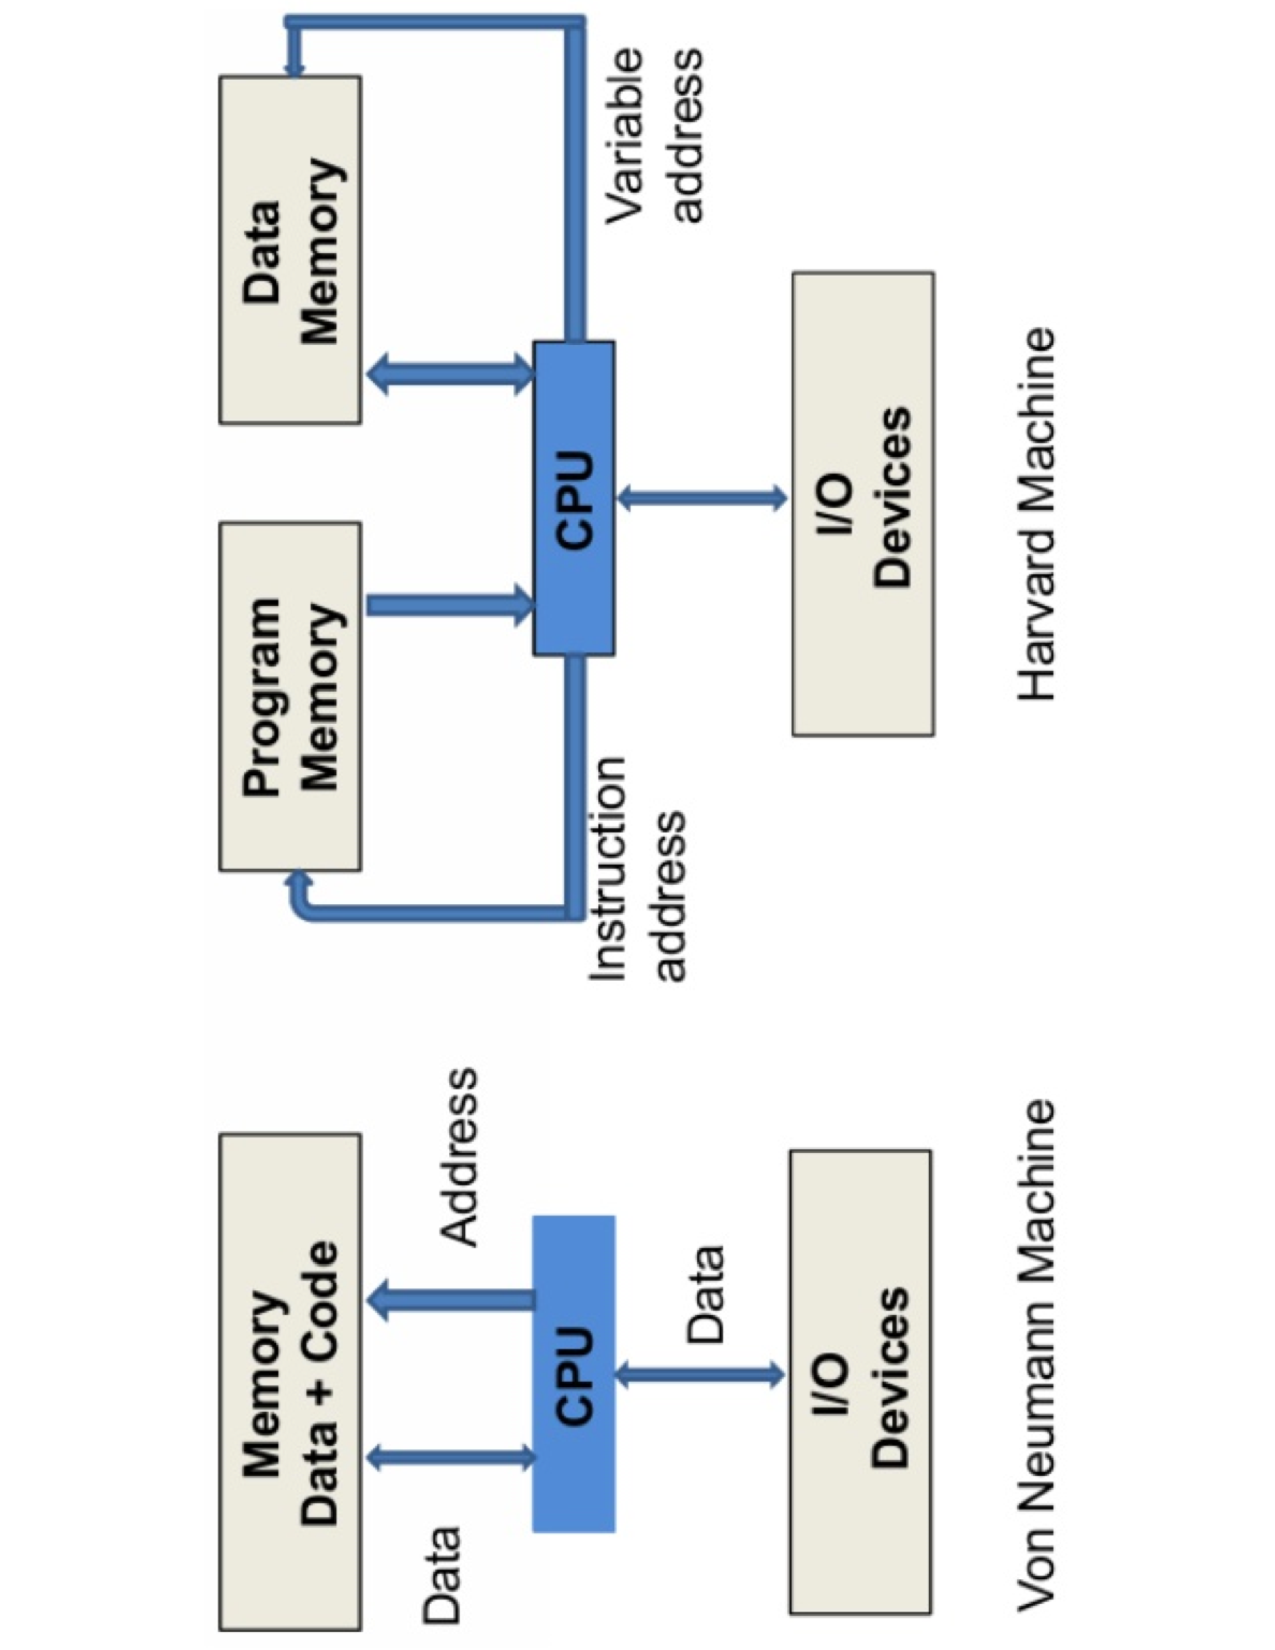
\includegraphics[angle=270,width=10cm,trim=50 1 50 1,clip]{./Figures/cpu/vonneumann.pdf}
  \rule{35em}{0.5pt}
  \caption[vn]{Les architectures de Von Neumann et Harvard}
  \label{fig:vn}
\end{figure}

\subsection{Pile}
La gestion d'une pile mémoire est essentielle au fonctionnement d'un programme. Elle s'occupe de stocker temporairement l'information pour gérer:
\begin{itemize}[label=\textbullet,font=\small]
\item Le changement de contexte comme lors d'une interruption ou d'un appel de fonction
\item Le stockage des paramètres de fonction
\item Le stockage des variables locales
\item Certaines variables lors de branchements multiples (switch-case)
\end{itemize}
La pile peut être de type matérielle ou logicielle, dans le premier cas elle aura un nombre limité de registres et dans le deuxième elle sera juste une zone de la mémoire RAM.

\section{Registres à usages spécifiques}
Parmi tous les registres de la machine, il y en a trois qui sont essentiels au bon fonctionnement de la machine et qui sont accessibles au programmeur.

\subsection{Registre d'état}
C'est le registre contenant l'état de la machine, appelé SR (Status Register), qui peut contenir les informations suivantes:
\begin{itemize}
\item Statut de la dernière opération arithmétique sur 4 bits (CVNZ)
\item Interruptions activées ou non (1 bit)
\item Mode low power 2-3 bits
\item Configuration des horloges 2-3 bits
\end{itemize}
La longueur du registre est normalisée par rapport à la largeur du bus de données.

Les bits de statut arithmétique sont utilisés pour des tests ou pour détecter des dépassements de capacité:\\
C: Carry, c'est l'indication qu'une retenue a été générée\\
V: oVerflow, c'est l'indication d'un dépassement lors du calcul avec des nombres signés\\
N: Negative, c'est l'indication d'un résultat négatif\\
Z: Zero, c'est l'indication d'un résultat nul

\subsection{Pointeur de programme}
Registre contenant l'adresse mémoire de l'instruction en cours appelé PC (Program Counter). La longueur de ce registre est celui de la largeur du bus d'adresses. Ce registre est incrémenté, après chaque instruction, d'un entier qui correspond à la longueur de l'instruction précédente.

\subsection{Pointeur de pile}
Registre contenant l'adresse mémoire du dessus de la pile appelé SP (Stack Pointer). La longueur de ce registre est celui de la largeur du bus d'adresses. Ce registre est incrémenté, après chaque empilement/désempilement, d'un entier qui correspond à la longueur de l'information stockée dans la pile.

\section{Cycle des instructions}
Pour analyser en détail le fonctionnement du processeur soumis à une instruction, on va diviser le processus en cinq parties:

\begin{enumerate}
\item Recherche de l'instruction (IF: Instruction Fetch)
\item Décodage de l'instruction (ID: Instruction Decode)
\item Recherche des opérandes (OF: Operand Fetch)
\item Exécution de l'instruction (EX: EXecute)
\item Écriture du résultat (WR: Write Register ou WB: Write Back)
\end{enumerate}

\newpage
\subsection{Recherche de l'instruction}
Dans cette phase, on doit amener l'instruction de la mémoire vers un registre d'instruction dans le séquenceur. La première chose à faire c'est de placer sur le bus d'adresses la valeur du pointeur de programme (Le pointeur de programme contient l'adresse de la ligne du programme). Cette adresse est alors dirigée sur la mémoire qui retourne la valeur qu'elle contient sur le bus de données (fig. \ref{fig:instr1}).

\begin{figure}[htb]
  \centering
  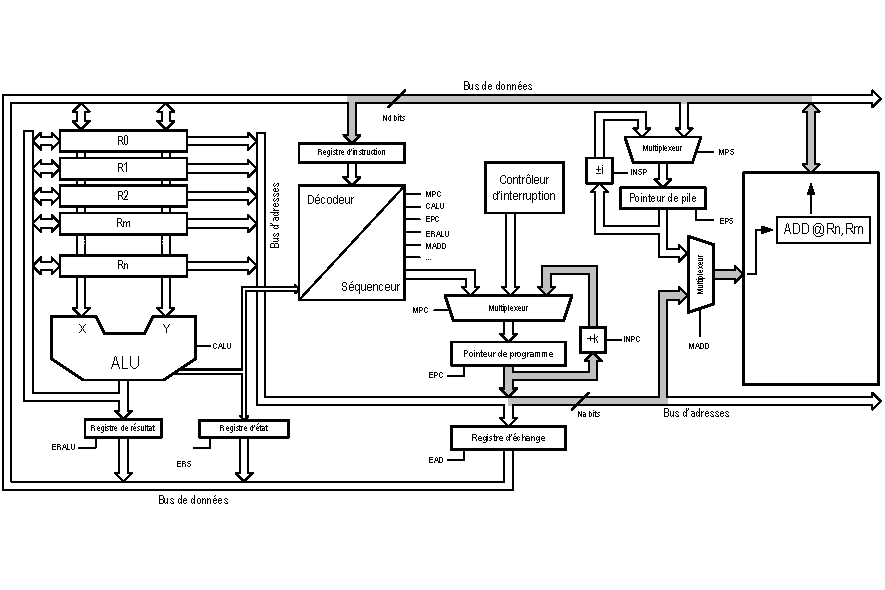
\includegraphics[angle=0, width=15cm, trim=0 30 0 30,clip]{./Figures/cpu/instruction1.pdf}
  \rule{35em}{0.5pt}
  \caption[instr1]{Recherche de l'instruction}
  \label{fig:instr1}
\end{figure}

\newpage
\subsection{Décodage de l'instruction}
Dés que l'instruction est arrivée dans le séquenceur, il peut la décoder en lisant d'abord l'opcode qui identifie l'instruction à effectuer par exemple add (fig. \ref{fig:opcode1}). Deuxièmement, il lit la méthode d'adressage utilisée pour trouver l'endroit de la source et de la destination. 

\begin{figure}[htb]
  \centering
  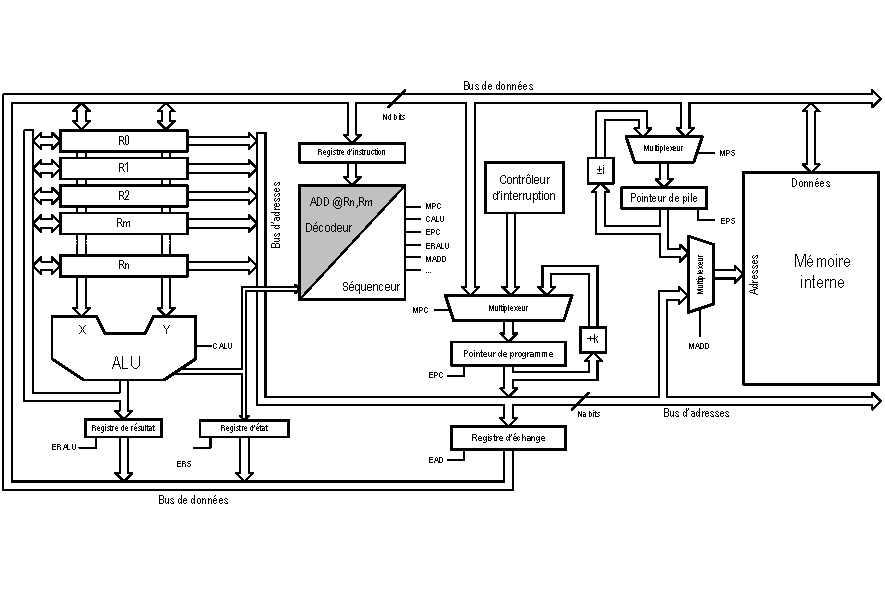
\includegraphics[angle=0, width=15cm, trim=0 30 0 30,clip]{./Figures/cpu/instruction2.pdf}
  \rule{35em}{0.5pt}
  \caption[instr2]{Décodage de l'instruction}
  \label{fig:instr2}
\end{figure}

\begin{figure}[htb]
  \centering
  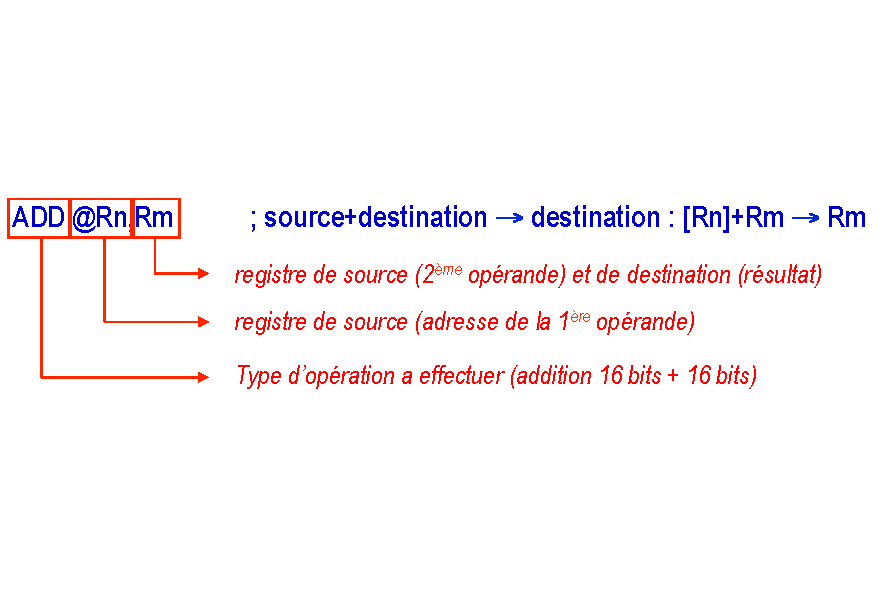
\includegraphics[angle=0, width=12cm, trim=0 90 0 90,clip]{./Figures/cpu/opcode1.pdf}
  \rule{35em}{0.5pt}
  \caption[opcode1]{Exemple d'instruction assembleur}
  \label{fig:opcode1}
\end{figure}

\begin{figure}[H]
  \centering
  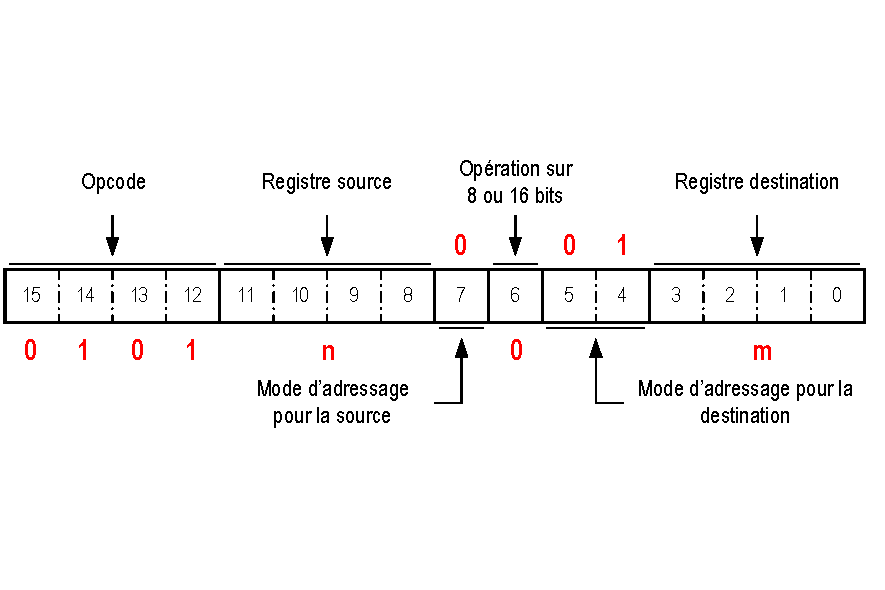
\includegraphics[angle=0, width=14cm, trim=0 70 0 70,clip]{./Figures/cpu/opcode2.pdf}
  \rule{35em}{0.5pt}
  \caption[opcode2]{Exemple de codage d'une instruction}
  \label{fig:opcode2}
\end{figure}

\newpage
\subsection{Recherche des opérandes}
Après décodage, le séquenceur entre en oeuvre et va chercher les opérandes suivant le mode d'adressage utilisé. Si l'adressage est direct, les registres internes au chemin de données sont activés et présentent leurs valeurs aux entrées de l'ALU. Si l'adressage est indirect, le séquenceur place la valeur contenue dans un registre sur le bus d'adresse. Ensuite la valeur en mémoire située à cette adresse est placée sur le bus de donnée pour atteindre finalement l'entrée de l'ALU.

\begin{figure}[htb]
  \centering
  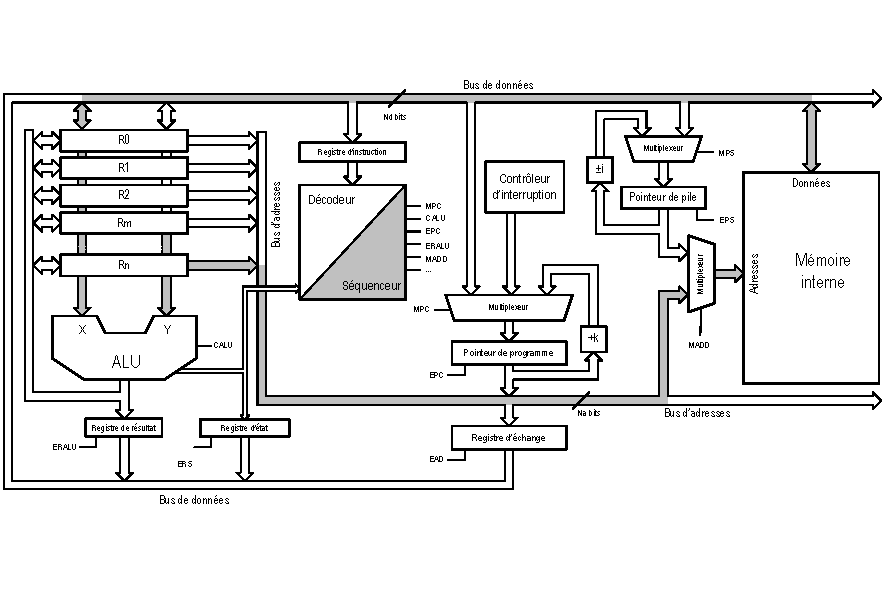
\includegraphics[angle=0, width=15cm, trim=0 30 0 30,clip]{./Figures/cpu/instruction3.pdf}
  \rule{35em}{0.5pt}
  \caption[instr3]{Recherche des opérandes}
  \label{fig:instr3}
\end{figure}
 
\subsection{Exécution de l'instruction}
A partir du moment ou les données sont présentent aux deux entrées de l'ALU, le séquenceur commande l'exécution de l'opération. Suivant la complexité de l'opération, l'exécution se décomposera en plusieurs sous opérations.

\begin{figure}[htb]
  \centering
  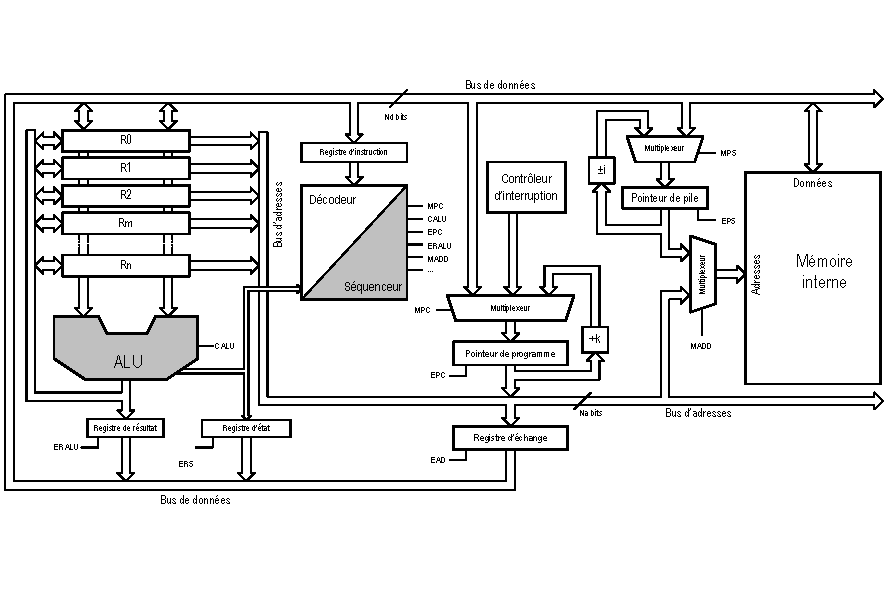
\includegraphics[angle=0, width=15cm, trim=0 30 0 30,clip]{./Figures/cpu/instruction4.pdf}
  \rule{35em}{0.5pt}
  \caption[instr4]{Exécution de l'instruction}
  \label{fig:instr4}
\end{figure}

\newpage
\subsection{Écriture du résultat}
Après le calcul de l'ALU, le résultat est placé dans le registre de destination. Le registre d'état est aussi mis à jour en même temps. Ce registre nous donne les informations suivantes:

\begin{itemize}[label=\textbullet,font=\small]
\item Indication d'une retenue: C (pour Carry)
\item Indication d'un dépassement: V (pour oVerflow)
\item Indication d'un résultat négatif: N (pour Negative)
\item Indication d'un résultat nul: Z (pour Zero)
\end{itemize}

Grâce à ces informations, nous pouvons programmer en utilisant des conditions. Par exemple, pour tester lorsque qu'une boucle for arrive à zéro.

\begin{figure}[htb]
  \centering
  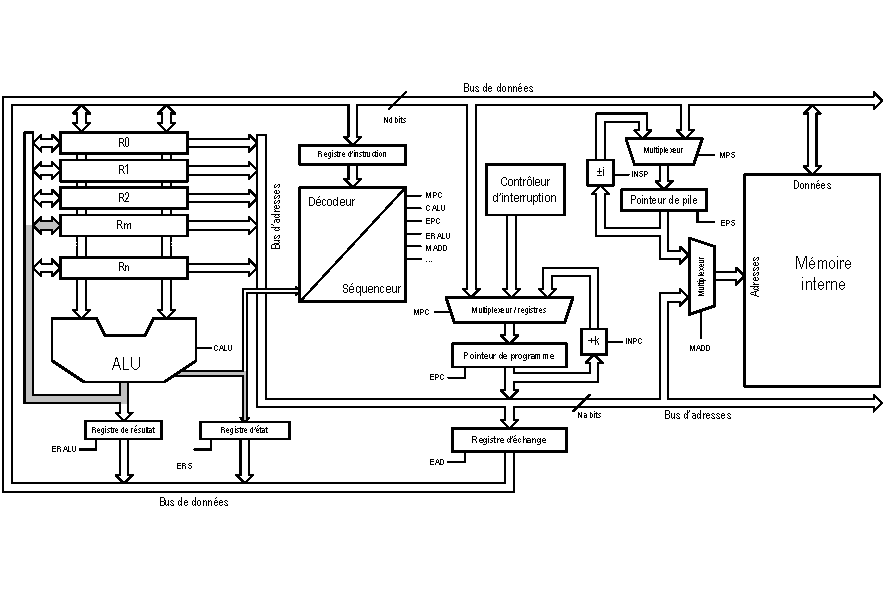
\includegraphics[angle=0, width=15cm, trim=0 30 0 30,clip]{./Figures/cpu/instruction5.pdf}
  \rule{35em}{0.5pt}
  \caption[instr5]{Écriture du résultat}
  \label{fig:instr5}
\end{figure}

\newpage
\section{Séquenceur des instructions}
Le séquenceur est un composants clé qui à pour but de gérer le bon fonctionnement du processeur. Il prend en compte les temps d'exécutions de chaque sous composants. On peut le réaliser de deux manières différentes: i) cablé (fig. \ref{fig:sc}), c-à-d par des fonctions logique séquentielles ou ii) microprogrammé (fig. \ref{fig:sm}), qui signifie qu'il peut être reconfiguré.
 
\begin{figure}[htb]
  \centering
  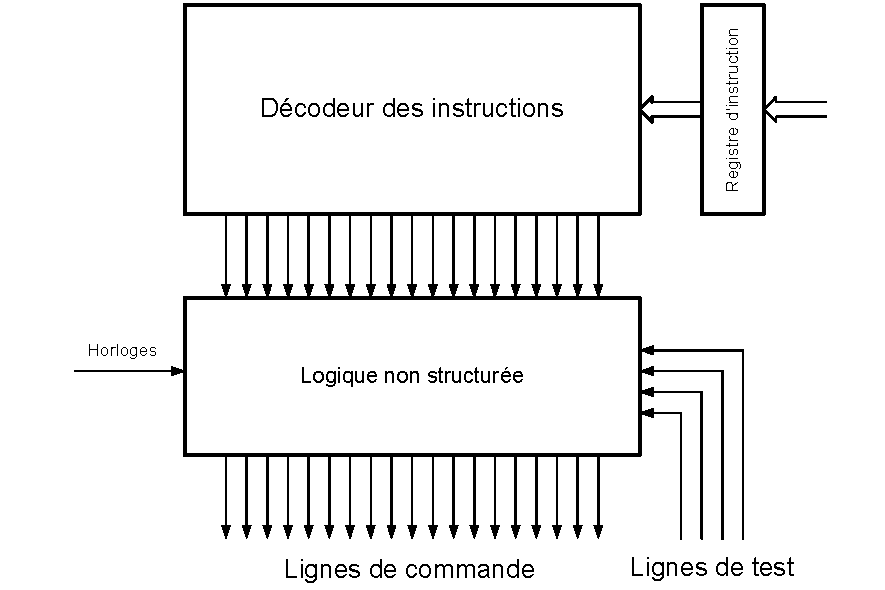
\includegraphics[angle=0, width=12cm]{./Figures/cpu/Sequenceur1.pdf}
  \rule{35em}{0.5pt}
  \caption[sc]{Séquenceur câblé}
  \label{fig:sc}
\end{figure}

\begin{figure}[htb]
  \centering
  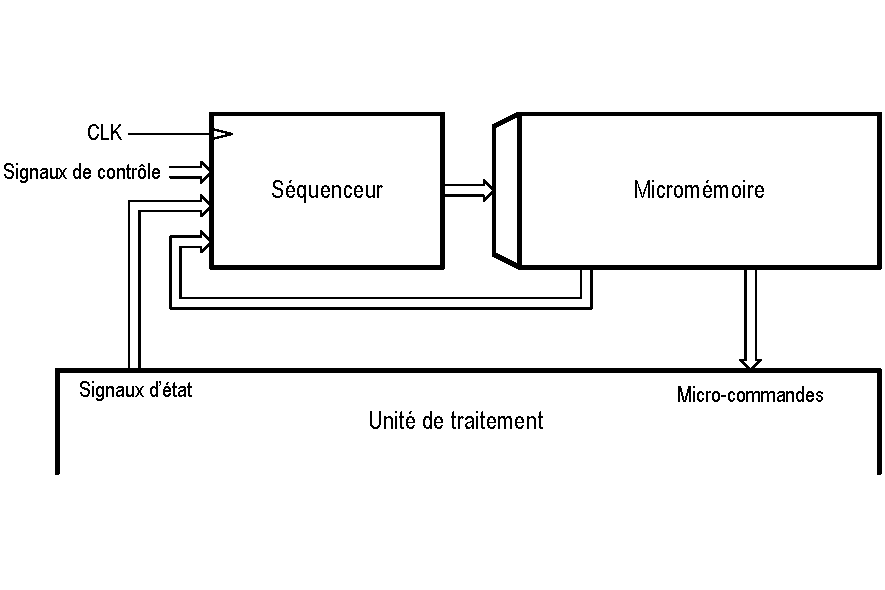
\includegraphics[angle=0, width=12cm, trim=0 40 0 40,clip]{./Figures/cpu/Sequenceur2.pdf}
  \rule{35em}{0.5pt}
  \caption[sm]{Séquenceur microprogrammé}
  \label{fig:sm}
\end{figure}

\begin{figure}[htb]
  \centering
  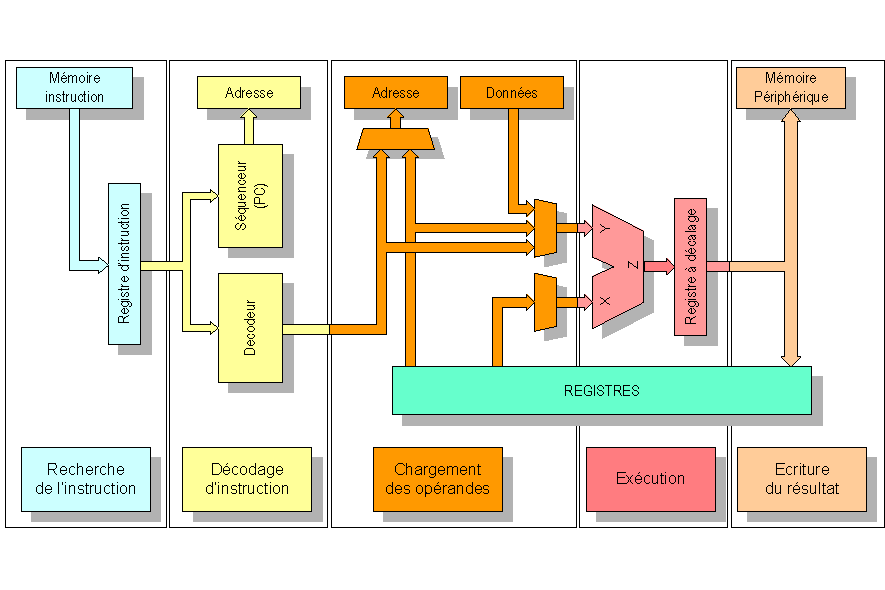
\includegraphics[angle=0, width=12cm, trim=0 20 0 20,clip]{./Figures/cpu/withoutpipeline1.pdf}
  \rule{35em}{0.5pt}
  \caption[flux1]{Flux des instructions sans pipeline}
  \label{fig:flux1}
\end{figure}

\begin{figure}[htb]
  \centering
  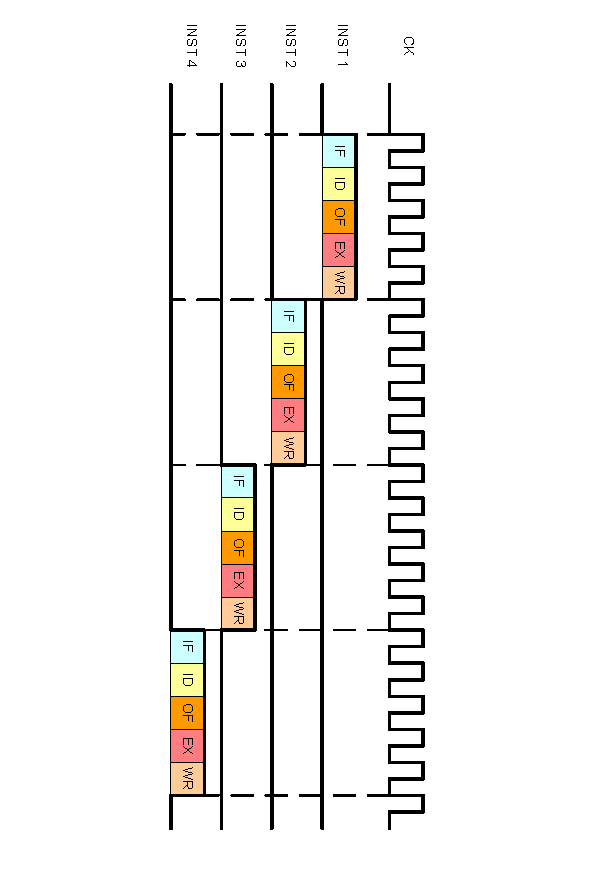
\includegraphics[angle=90, width=12cm,trim=60 1 60 1,clip]{./Figures/cpu/wpipeline2.pdf}
  \rule{35em}{0.5pt}
  \caption[flux2]{Flux des instructions sans pipeline}
  \label{fig:flux2}
\end{figure}
 
\section{Pipeline du cycle des instructions}
Les cinq étapes citées auparavant doivent être exécutées à la suite ce qui donne un cycle minimum de cinq coup d'horloges pour exécuter une instruction (fig. \ref{fig:flux2}). On désire donc commencer une nouvelle instruction dés que possible c-à-d dés qu'un étape est terminée ((fig. \ref{fig:flux4})).

Pour se faire, on intercale des registres entre les différentes phases du processus ((fig. \ref{fig:flux3})). Ceci permet d'isoler chaque phase et ainsi de permettre la réutilisation des phases à chaque cycle d'horloge du processeur.

\begin{figure}[htb]
  \centering
  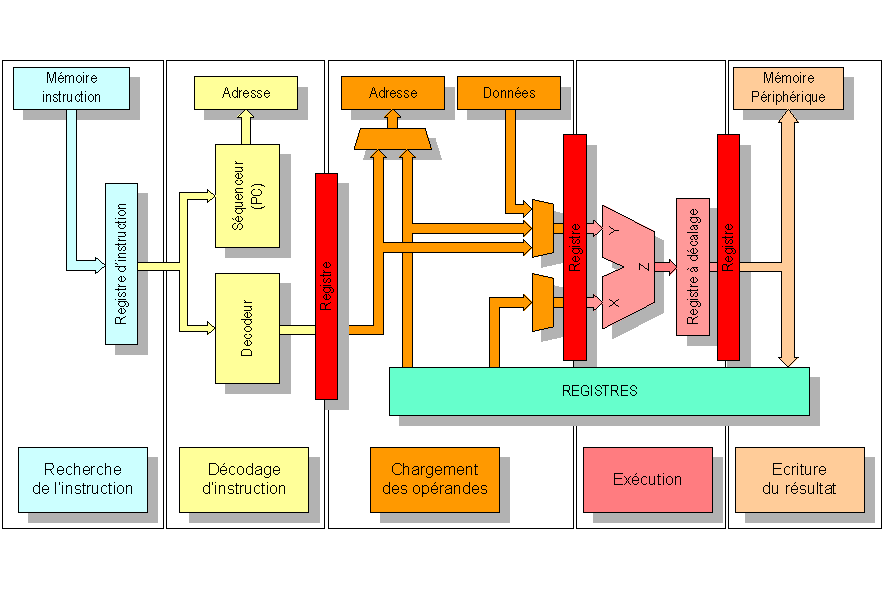
\includegraphics[angle=0, width=12cm, trim=1 20 1 20,clip]{./Figures/cpu/withpipeline1.pdf}
  \rule{35em}{0.5pt}
  \caption[flux3]{Flux des instructions avec pipeline}
  \label{fig:flux3}
\end{figure}

\begin{figure}[htb]
  \centering
  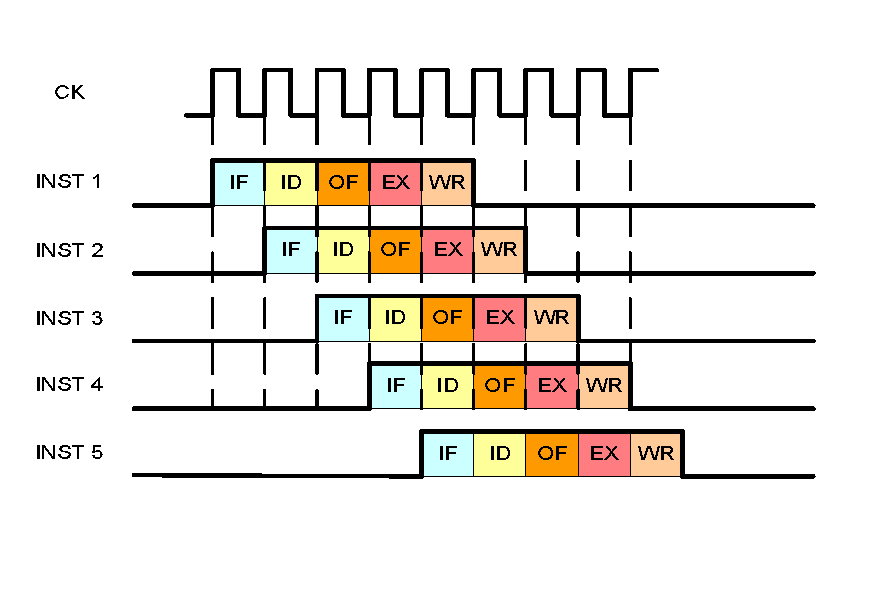
\includegraphics[angle=0, width=12cm, trim=1 30 1 30,clip]{./Figures/cpu/withpipeline2.pdf}
  \rule{35em}{0.5pt}
  \caption[flux4]{Flux des instructions avec pipeline}
  \label{fig:flux4}
\end{figure}

Certaines opérations sont plus longues que d'autres ce qui fait que l'horloge doit être ajustée pour l'étape la plus lente. Pour éviter de devoir ralentir l'horloge du cpu on peut ajouter des niveaux de pipeline pour accélérer le processeur. Par exemple un multiplieur prendra plus de temps qu'un additionneur, il est donc judicieux de réaliser le multiplieur avec plusieurs étages de pipeline. 

\section{Processeur superscalaire}
Un processeur capable d'exécuter plusieurs instructions en parallèle est dit superscalaire. Ce n'est pas un ensemble de processeurs mais un seul CPU avec plusieurs ALU qui peut aussi avoir plusieurs décodeurs/séquenceurs. On utilise aussi la terminologie anglo-saxone "dual-issue" pour un processeur qui peut exécuter deux instructions en parallèle et "multiple-issue" pour un processeur qui peut en exécuter plusieurs. Un processeur qui peut exécuter une seule instruction par cycle d'horloge est donc appelé "single-issue", c'est le cas de la plupart des micro-contrôleurs. 

Un processeur qui possède plusieurs ALU mais pas plusieurs décodeurs d'instructions est dit avec pipeline superscalaire. L'ARM cortex M7, par exemple, possède cinq pipelines: deux ALU entières, un pour les opération mémoire, un pour faire des multiplications/accumulations et un pour le calcul en virgule flottante. Cela permet d'équilibrer les opérations qui ont des temps d'exécutions différents tel que le calcul en virgule flottante par rapport au calcul entier. Par exemple, une instruction flottante prend 4 étages de pipeline alors qu'une instruction entière en prend 2. Donc si on place une instruction flottante suivie par une instruction entière, on a bien deux instructions qui s'exécutent en parallèle. L'instruction entière se terminera un cycle avant l'instruction flottante.

La présence de processeurs de plus en plus puissants dans les micro-contrôleurs est inévitable. Ceci est dû à plusieurs facteurs: 
\begin{enumerate}
\item La densité d'intégration des technologies CMOS => plus de transistors disponibles
\item La réduction de la consommation dynamique liée aux circuits plus petits
\item La vitesse et complexité des interfaces de communications, par exemple l'USB
\item La complexité des périphériques disponibles, par exemple les afficheurs
\end{enumerate}

On peut donc s'attendre à trouver des microcontroleurs qui s'approchent des fonctionnalités d'un ordinateur de base.


